% !TEX encoding = UTF-8
% !TEX TS-program = pdflatex
% !TEX root = ../Tesi.tex
% !TEX spellcheck = en-EN

%************************************************
\chapter{Artificial Neural Network}
\label{cap:ann}
%************************************************

\section{Regression statistic}
\label{sec:regressionstatistic}

\section{ANN intro}
\label{sec:annintro}

An Artificial Neural Network (\acs{ANN}) is a powerful modelling technique, 
that is based on non-linear functions (Haykin \cite{RefWorks:158}). 

\improvement{Add some more details from Haykin introduction}

The biological inspiration for artificial neural networks can be seen in Fig.
\ref{fig:049neuron1}

\begin{figure}[!htb]
\centering
\includegraphics[width=.50\columnwidth]{images/049neuron1}
\caption[Biological inspiration 2]{Biological inspiration 2 for the Artificial
Neural Networks: a human neuron with the incoming electric signals
\cite{RefWorks:158}.}
\label{fig:049neuron1}
\end{figure}

In this work, we first used the \acs{ANN} to fit the \acs{DEM} numerical simulation
data, and then to process a vast number of parameters combinations. 
\acs{ANNs} map combinations of input data to convenient outputs (fitting). 
There is a variety of \acs{ANNs} available; important for our context were the
Feedforward ($FF$) and the Radial basis function ($RBF$). 
For $FF-NN$, 
numerous training algorithms are available. The most common are based on
backpropagation, e.g., Levenberg-Marquardt, Bayesian regulation and the scaled
conjugate gradient.

\section{Perceptron}
\label{sec:perceptron}

The basic element of an artificial neural network is the perceptron, see Fig.
\ref{fig:064perceptron}\\
\improvement{Add some more details about the perceptron from Haykin}
\improvement{explain feed forward here}
\begin{figure}[!htb]
\centering
\includegraphics[width=.80\columnwidth]{images/064perceptron}
\caption[Perceptron scheme]{Perceptron scheme.}
\label{fig:064perceptron}
\end{figure}

\section{Multilayer}
\label{sec:multilayer}

\improvement{Add some more details about the multilayer from Haykin}
The double moon, see Fig. \ref{fig:063doublemoon}, is the most classical
example  to illustrate why a single neuron is not capable to handle a
nonlinear problem.\\
\improvement{better and more detailed explanation about the double moon}
\begin{figure}[!h]
\centering
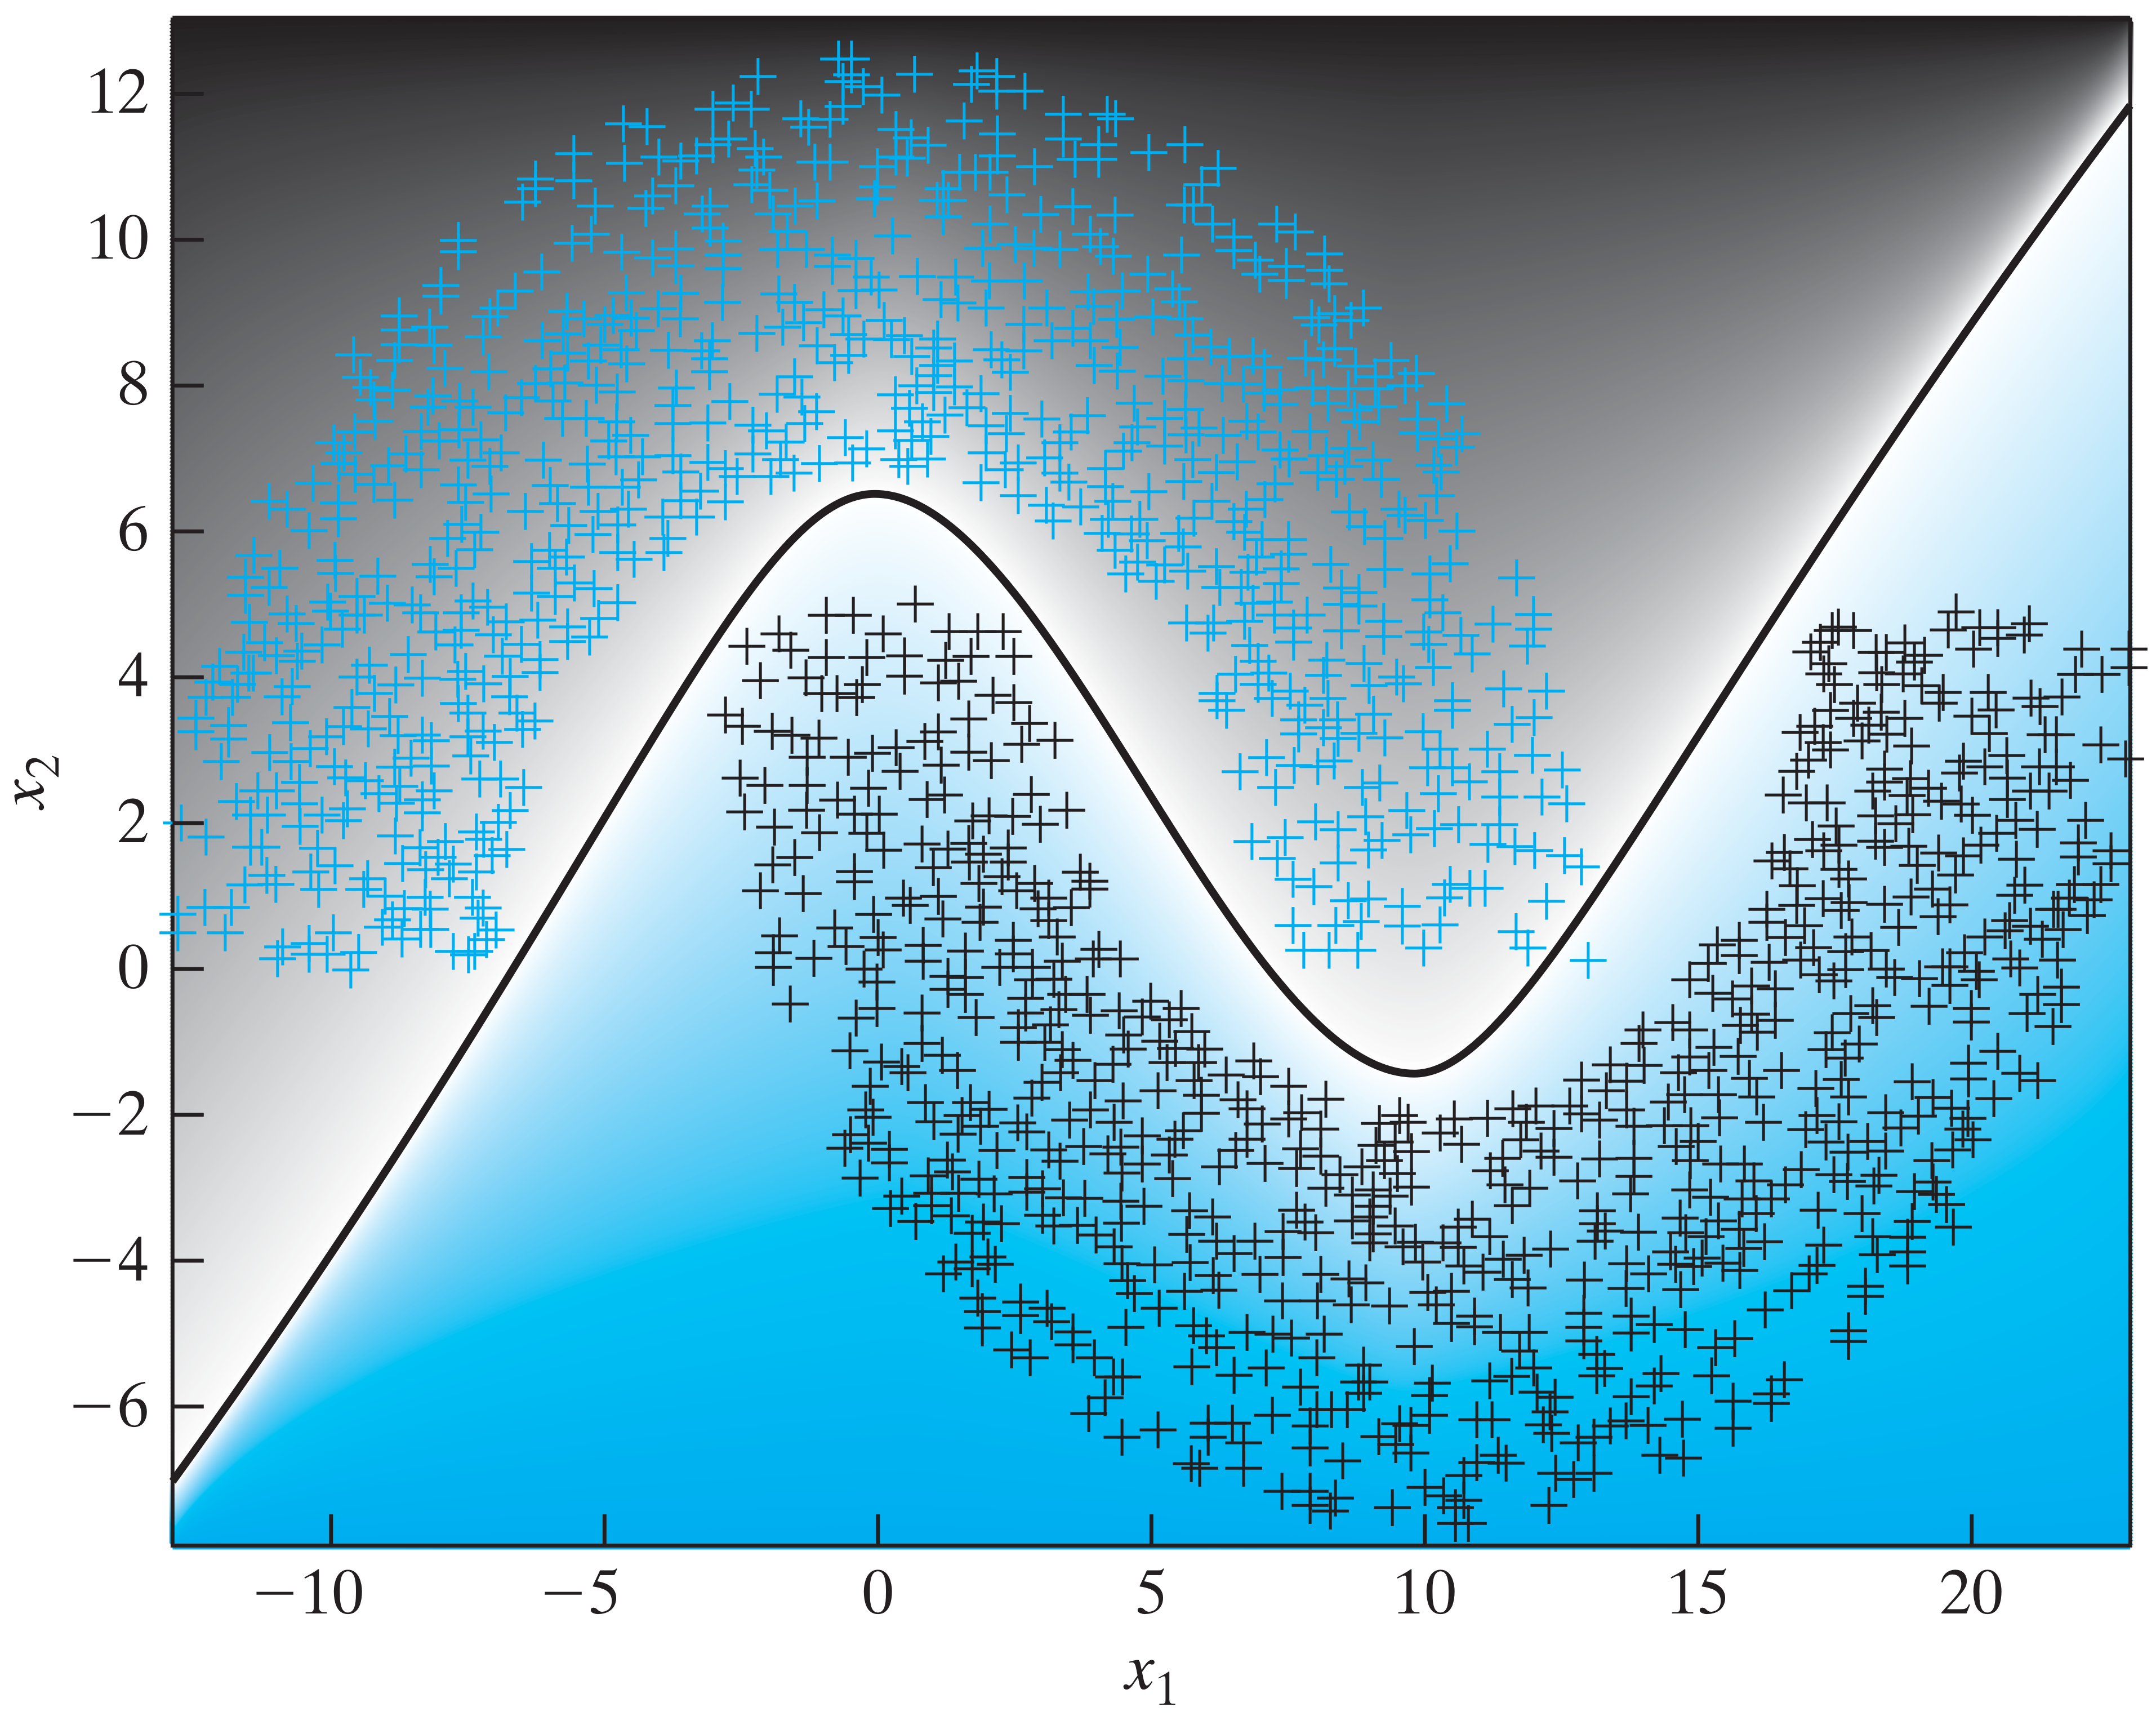
\includegraphics[width=.70\columnwidth]{images/063doublemoon}
\caption[Double moon classification problem]{Double moon classification
problem \cite{RefWorks:158}.}
\label{fig:063doublemoon}
\end{figure}

\section{Backpropagation algorithm}
\label{sec:backpropagationalgorithm}

To be able to handle non-linearly separable data, the standard linear perceptron
\acs{ANN} was modified to obtain \textit{FF Multilayer Perceptron Neural Networks
(MLPNN)}.
Here, each processing unit or node (neuron) possesses a nonlinear activation function. 
They are interconnected to form layers that are also interlinked. 
The validity of the $MLPNN$, with a backpropagation reinforcement learning 
training algorithm (scaled conjugate gradient), has been demonstrated in the 
literature, see Haykin \cite{RefWorks:158}. Several scientists 
\cite{RefWorks:161, RefWorks:166, RefWorks:167, RefWorks:168, RefWorks:169,
RefWorks:170, RefWorks:178, RefWorks:179} have employed \acs{ANNs} to model
the mechanical properties of materials.

\section{Cross validation}
\label{sec:crossvalidation}

\begin{enumerate}
  \item{training samples set}
  \item{generalization samples set (or validation, or for early stopping)}
  \item{test samples set}
\end{enumerate}

\section{Supervised learning and optimization}
\label{sec:supervisedlearningandoptimization}

\begin{itemize}
  \item{conjugate gradient \improvement{add details}}
  \item{quasi-Newton}
  \item{Levenberg-Marquardt}
\end{itemize}

\section{Our ANNs}
\label{sec:ouranns}

\wrong{change subsection title}

Following the best practice suggested by Vaferi et al. \cite{RefWorks:150}, we
used $MLPNN$.
Further, the quality of the \acs{ANN} data had to be examined critically. 
Haykin \cite{RefWorks:158} 
suggested considering the quality of (a) \acs{ANN} training process and (b) the
subsequent data generation based on the inputs provided.
Task (a) is particularly important
when dealing with experimental training data, and
usually addressed
by noise-corrupted pattern calibration
and by comparison with standard statistical methods.
However, our training pool was numerical and extensive, 
and the particles in our simulations were inserted using a random
seed value.
For vast amounts of training data, the effect of noise-corrupted patterns is
negligible, see Haykin \cite{RefWorks:158}.
We used the Bayesian linear and the Gaussian non linear regressions to further
assess the quality of the training.
Thus, in our work task (b) was more challenging.
Once trained, the \acs{ANN} were fed
combinations of \acs{DEM} parameters. 
We tried different methods to generate these combinations. 
Our first attempt consisted of assigning parameters to the investigated
variables in even increments from the minimum to the maximum values. 
For example, the \acs{CoR} ranged from 0.5 to 0.9, and thus the first value was
0.5, the second 0.508163, and so on.
To increase generalization, we decided to follow a different approach: 
random value generators created the number of required values in the defined
ranges for each parameter investigated.
These were combined and used as input.\\
